% Created 2022-07-05 Tue 08:21
% Intended LaTeX compiler: xelatex
\documentclass[11pt,twoside,landscape]{article}
\usepackage{graphicx}
\usepackage{longtable}
\usepackage{wrapfig}
\usepackage{rotating}
\usepackage[normalem]{ulem}
\usepackage{amsmath}
\usepackage{amssymb}
\usepackage{capt-of}
\usepackage{hyperref}
\usepackage{subcaption}
\usepackage[newfloat]{minted}
\usepackage{color}
\usepackage{listings}
\usepackage[top=2cm,bottom=2cm,right=2cm,left=2cm,landscape]{geometry}
\usepackage{multicol}
\usepackage{enumitem}
\usepackage{fancyhdr}
\usepackage{caption}
\usepackage{algorithm}
\usepackage{algpseudocode}
\usepackage{float}
\setlist{noitemsep}
\setlength{\parindent}{0pt}
\setlength{\columnseprule}{0.2pt}
\definecolor{mygreen}{rgb}{0,0.6,0}
\definecolor{mygray}{rgb}{0.5,0.5,0.5}
\definecolor{mymauve}{rgb}{0.58,0,0.82}
\lstset{ backgroundcolor=\color{white}, basicstyle=\footnotesize, breaklines=true, captionpos=b, commentstyle=\color{mygreen}, escapeinside={\%*}{*)},keywordstyle=\color{blue}, stringstyle=\color{mymauve},}
\author{Olivier Lischer}
\date{\today}
\title{ParProg Summary}
\hypersetup{
 pdfauthor={Olivier Lischer},
 pdftitle={ParProg Summary},
 pdfkeywords={},
 pdfsubject={},
 pdfcreator={Emacs 28.1 (Org mode 9.5.4)}, 
 pdflang={English}}
\begin{document}

\pagestyle{fancy}
\fancyhf{}
\fancyhead[R]{ParProg-FS22}
\fancyhead[L]{Exam Summary}
\fancyfoot[CE,CO]{\leftmark}
\fancyfoot[R]{\thepage}
\fancyfoot[L]{Olivier Lischer}

\begin{multicols}{3}

\section{Synchronization Mechanism}
\label{sec:orgcf270f8}
\subparagraph{Lock \& Conditions} \
\label{sec:org5384be1}
{
\begin{center}
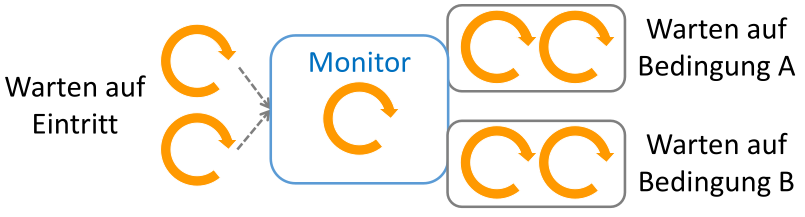
\includegraphics[width=.9\linewidth]{img/lock_and_conditions.png}
\end{center}
\captionof{figure}{Lock & Conditions}\label{fig:lock-and-conditions}
}

\lstset{language=java,label= ,caption= ,captionpos=b,numbers=none}
\begin{lstlisting}
public class WarehouseWithLockCondition {
    public WarehouseWithLockCondition(int capacity, boolean fair) {
	lock = new ReentrantLock(fair);
	nonEmpty = lock.newCondition();
	nonFull = lock.newCondition();
    }

    @Override
    public void put(int amount) throws InterruptedException {
	lock.lock();
	try {
	    // nonFull.await();
	    // nonEmpty.signalAll();
	} finally {
	    lock.unlock();
	}
    }

    @Override
    public void get(int amount) throws InterruptedException { /* code */ }
}
\end{lstlisting}

\subparagraph{Read-Write Locks} \
\label{sec:org1600164}
\lstset{language=java,label= ,caption= ,captionpos=b,numbers=none}
\begin{lstlisting}
var rwLock = new ReentrantReadWriteLock(true);
rwLock.readLock().lock();
// read-only accesses
rwLock.readLock().unlock();
rwLock.writeLock().lock();
// write (and read) accesses
rwLock.writeLock().unlock();
\end{lstlisting}
\subparagraph{CountdownLatch} \
\label{sec:org1bcb272}
\lstset{language=java,label= ,caption= ,captionpos=b,numbers=none}
\begin{lstlisting}
CountDownLatch waitForAll = new CountDownLatch(this.CARS);
protected void test() throws InterruptedException {
    waitForAll.countDown();
    waitForAll.await();
}
\end{lstlisting}
\subparagraph{Cyclic Barrier} \
\label{sec:orgfc5baaf}
\lstset{language=java,label= ,caption= ,captionpos=b,numbers=none}
\begin{lstlisting}
var gameRound = new CyclicBarrier(5);

/* 5 different players / threads */
while (true) gameRound.await();
\end{lstlisting}

\subparagraph{Rendez-Vous} \
\label{sec:orgff3da3c}
\begin{itemize}
\item Without exchange: \texttt{new CyclicBarrier(2);}
\item With exchange: \texttt{Exchanger.exchange(something)};
\end{itemize}
\section{Thread Pool}
\label{sec:org29b275b}
\subparagraph{Java} \
\label{sec:org7016310}
\lstset{language=java,label= ,caption= ,captionpos=b,numbers=none}
\begin{lstlisting}
var threadPool = new ForkJoinPool();
Future<Integer> future = threadPool.submit(() -> {
	int value = 1;
	return value;
});
Integer i = future.get();

class MyTask extends RecursiveTask<Integer> {
    boolean finished = false;
    @Override
    protected Integer compute() {
	if (finished) return 1;
	var left = new MyTask();
	var right = new MyTask();
	left.fork();
	right.fork();
	return left.join() + right.join();
    }
}
\end{lstlisting}
\subparagraph{.NET} \
\label{sec:org046a67c}
\lstset{language=csharp,label= ,caption= ,captionpos=b,numbers=none}
\begin{lstlisting}
Task task1 = Task.Run(() => { /* Do some stuff */ });
task1.Wait(); // blocking

// Task with return value
Task task2 = Task.Run(() => { return 3;});
Console.Write(task.Result); // blocking

// Task with Sub Tasks
Task.Run(() => {
    var left = Task.Run(() => Count(leftPart));
    var right = Task.Run(() => Count(rightPart));
    int result = left.Result + right.Result;
    return result;
});

// Parallele Statements
Parallel.Invoke(
    () => MergeSort(l, m),
    () => MergeSort(m, r)
);

// Parallel Loop
Parallel.ForEach(list, file => Convert(file));

// Parallel For - only if iterations are indepentend
Parallel.For(0, array.Length, i => DoComputation(array[i]));
\end{lstlisting}
\section{Async}
\label{sec:org3f170ce}
\subparagraph{Continuation} \
\label{sec:org102eba1}
Exception in Fire \& Forget are ignored.
To handle exception you have to wait synchrony for finishing the task.

\lstset{language=csharp,label= ,caption= ,captionpos=b,numbers=none}
\begin{lstlisting}
Task.Run(task1).
    ContinueWith(task2).
    ContinueWith(task3).Wait();
Task.WhenAll(task1, task2).
    ContinueWith(continuation).Wait();
Task.WhenAny(task1, task2).
    ContinueWith(continuation).Wait();
\end{lstlisting}
\section{Memory Modell}
\label{sec:org6fb918f}
\subparagraph{Atomicity} \
\label{sec:orgbaa57b0}
Single reads / writes are atomic for:
\begin{itemize}
\item primitive data types until 32 bits
\item object references
\item long and double only with the \texttt{volatile} keyword
\end{itemize}
\subparagraph{Visibility} \
\label{sec:org5aba735}
Java guaranties the following visibility:
\begin{itemize}
\item changes before release are visible at acquire
\item changes until write are visible at read
\item the thread sees the correct start values and Join the output of the thread
\item initialization of final variables (only relevant if you get the object from a data race!)
\end{itemize}

\subparagraph{Ordering} \
\label{sec:org8cf4630}
The order of the visibility is the same as in visibility.
Additional:
\begin{itemize}
\item synchronization instructions are never reordered to each other
\item Lock/Unlock, volatile, thread start / join are never reordered
\item if everything is a synchronization mechanism than we talk about total order
\end{itemize}

\section{GPU}
\label{sec:org57a7419}
\begin{description}
\item[{latency}] how long does it take to execute a single instruction / operation
\item[{throughput}] number of instructions / operations completed per second
\end{description}
\subparagraph{Arithmetic Intensity} \
\label{sec:org15c74ee}

\begin{equation}
  \begin{align}
    &t_c > t_m \\
    &\frac{ops}{BW_c} > \frac{bytes}{BW_m} \\
    &\frac{ops}{bytes} > \frac{BW_C}{BW_m} \\
    &\text{Arithmetic intensity} = \frac{BW_c}{BW_m}
  \end{align}
\end{equation}

\subparagraph{Thermilogy} \
\label{sec:org9e788aa}
{
\begin{center}
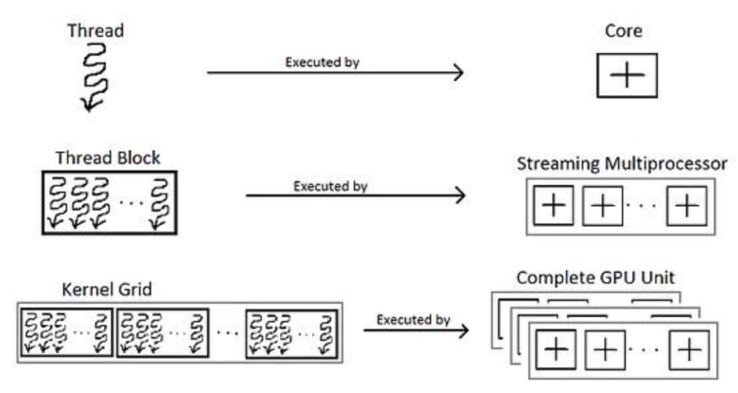
\includegraphics[width=.9\linewidth]{img/cuda_to_gpu_analogy.png}
\end{center}
\captionof{figure}{CUDA concepts on the GPU}\label{fig:cuda-concepts-on-the-gpu}
}

\subparagraph{Classification} \
\label{sec:orgc7b804e}

{
\begin{center}
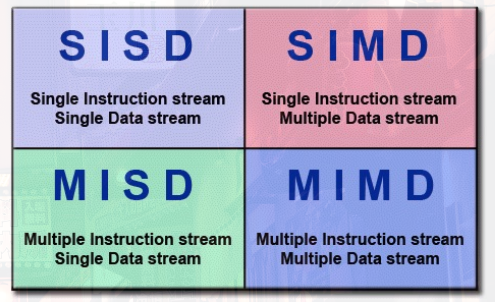
\includegraphics[width=.9\linewidth]{img/flynn_classical_taxonomy.png}
\end{center}
\captionof{figure}{Flynn's Classical Taxonomy}\label{fig:flynns-classical-taxonomy}
}

\section{Laws}
\label{sec:orgbed84da}
\subparagraph{Amdahls's law} \
\label{sec:org4b33949}
\begin{equation}
  \text{SpeedUp} = \frac{1}{s + \frac{p}{N}}
\end{equation}

\subparagraph{Gutafson's law} \
\label{sec:orgc312a87}
\begin{description}
\item[{s}] serial part
\item[{p}] parallel part
\item[{N}] number of processes
\end{description}
\begin{equation}
\text{SpeedUp} = s + p \cdot N = s + (1-s) \cdot N
\end{equation}



\end{multicols}
\end{document}